\documentclass{slide}

\title{Architectural Decision Records}
\subtitle{CSSE6400}
\author{Richard Thomas}
\date{\week{2}}

\usepackage{languages}
\usepackage{changepage}

\hypersetup{
    colorlinks=true,
    linkcolor=violet,
    filecolor=purple,      
    urlcolor=blue,
    citecolor=black,
}

\begin{document}

\maketitle


\begin{frame}{Developer Reaction to Reading Software Architecture Documentation}

\begin{figure}
    \href{https://pixabay.com/vectors/computer-internet-unhappy-user-1295358/}{
\includegraphics[width=0.9\textwidth]{images/frustration.png}}
\end{figure}

\end{frame}


\questionanswer{How do you know why certain decisions were made in the architectural design?}
{\highlight{Architectural Decision Records (ADRs)}}


\begin{frame}{Record Decisions that Influence}

\Large{
\begin{itemize}
    \item \highlight{Structure} of the architecture.
    \item Delivery of \highlight{quality attributes}.
    \item \highlight{Dependencies} between important parts of the architecture.
    \item \highlight{Interfaces} between important parts of the architecture.
    \begin{itemize}
        \large{\item or external interfaces}
    \end{itemize}
    \item \highlight{Principles} about implementation techniques or platforms.
\end{itemize}
}

\end{frame}


\questionanswer{Why ADRs?}
{My code will defeat the architectural design,\\
if I do not know why it was designed that way.}

\point[ADRs]{Record a \highlight{single} decision.}

\point[ADRs]{Are \highlight{never} deleted.\\
Mark as \highlight{superseded} and link to new decision.}

\questionanswer{Where are ADRs documented?}
{Each decision is a separate file in the project repository.\footnote{See the \texttt{adrs} directory
in the \href{https://csse6400.uqcloud.net/resources/c4_model.zip}{C4 model} on the course website.}}


\begin{frame}{ADR Template \cite{nygard-adr}}

\Large{
\begin{description}
    \item[Title] Short phrase describing the decision.
    \item[Date] When the decision was made.
    \item[Status] Current status of the decision.
    \begin{itemize}
        \large{\item proposed, accepted, deprecated, superseded, rejected}
    \end{itemize}
    \item[Summary] Summarise the decision and its rationale.
    \item[Context] Describe the facts that influence the decision.
    \item[Decision] Explain how the decision will solve the problem.
    \item[Consequences] Impact of the decision.
    \begin{itemize}
        \large{\item what's easier to do}
        \large{\item what's harder to do}
    \end{itemize}
\end{description}
}

\end{frame}


\begin{frame}{ADR Example}

\begin{figure}
    \href{https://github.com/CSSE6400/software-architecture/blob/main/notes/views/c4_model/adrs/0001-independent-business-logic.md}
            {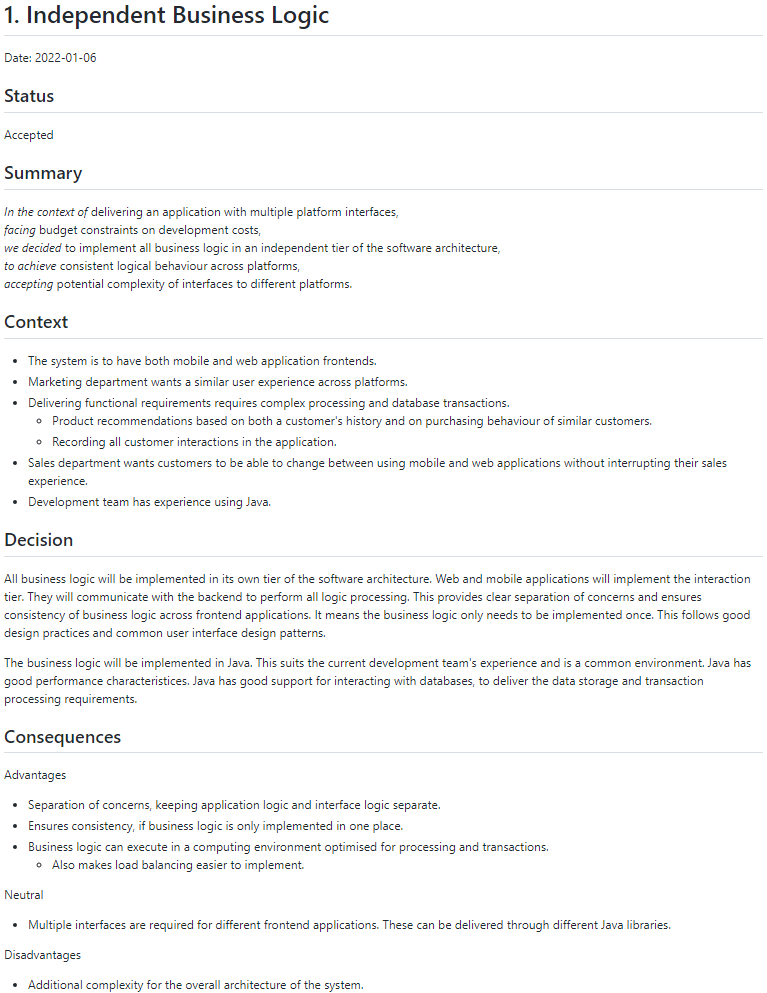
\includegraphics[height=\textheight]{images/adr-example.png}}
\end{figure}

\end{frame}


\point[Reading...]{``Architectural Decision Records'' Notes \cite{adr-notes}}


\begin{frame}

\begin{figure}
    \href{https://xkcd.com/2166/}{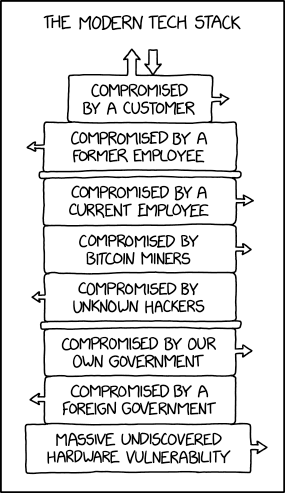
\includegraphics[height=\paperheight-11mm]{images/security_stack.png}}
    \caption{\url{https://xkcd.com/2166/}}
\end{figure}

\end{frame}


\references{articles,books}

\end{document}